% Final COSYNE revision, 18 October 2026.
% Two-page layout, revised Figure 1A, and peer-evaluation intuition beside N/D and V.
% Figure 2 is the author's manually edited Illustrator PDF, copied byte-for-byte.
% Body/cross-references updated for panels A-E; prior v9 source retained.
% 12 pt body, A4, 0.5 in margins, 10 pt captions/references, anonymous metadata.
\pdfminorversion=6
\documentclass[12pt,a4paper]{article}
\usepackage[margin=0.5in]{geometry}
\usepackage[T1]{fontenc}
\usepackage{times,amsmath,amssymb,graphicx,caption}
% Resolve figure paths both from the repository root and this subdirectory.
\graphicspath{{CoSyNe2027/}}
\usepackage[hidelinks]{hyperref}
\hypersetup{pdftitle={Why accurate neural predictions do not guarantee effective neural control},pdfauthor={},pdfsubject={COSYNE 2027: prediction-control dissociation},pdfkeywords={}}
\pagestyle{empty}
\setlength{\parindent}{0pt}
\linespread{0.90}
\setlength{\parskip}{0.5pt}
\AtBeginDocument{%
  \setlength{\abovedisplayskip}{1pt}%
  \setlength{\belowdisplayskip}{1pt}%
  \setlength{\abovedisplayshortskip}{1pt}%
  \setlength{\belowdisplayshortskip}{1pt}%
}
\setlength{\emergencystretch}{1.5em}
\captionsetup{font=footnotesize,labelfont=bf,labelsep=period,skip=2pt,hypcap=false}
\newcommand{\head}[1]{\par\noindent\textbf{#1}\enspace\ignorespaces}
\newcommand{\bh}{\hat\beta}
\newcommand{\bt}{\beta^\star}
\newcommand{\mb}{\bar\beta}
\begin{document}
{\large\bfseries Why accurate neural predictions do not guarantee effective neural control\par}

\textbf{Summary.}
%Encoding models of visual cortex can predict natural-image responses yet fail to generate images that control them. Motivated by experiments benchmarking control of ten models, we develop a regression theory of this dissociation. Prediction evaluates model on natural inputs, where estimation errors along low variance modes are concealed; control is evaluated on weight directions itself, with all error weighted equally. Random matrix theory shows how finite data and noise inflate model-predicted gain without increasing neural gain, leading to over-prediction and negative R2; and prediction-selected regularization need not prevent this failure. Feature transformations can preserve prediction while changing control arbitrarily, exposing a gradient-geometry factor whose nonlinear analogue correlates with biological control when held-out error is uninformative. The theory explains how poor generators recognize effective stimuli from other models. These results suggest how more data, noise reduction, and feature-gradient geometry can improve neural control.
Deep encoding models of visual cortex can effectively predict natural-image responses while failing to generate synthetic images that control neural firing (Prince \& Wang et al., 2026). Here we develop a regression theory to explain this dissociation. We consider linear regression from linear image features to noisy neural responses. We show that weight errors along low-variance directions of data matter little for accurate natural-image prediction but can severely distort predictions for synthetic images optimized through backpropagation to pixel space. Using random matrix theory, we then show how limited data and noise can cause models to overestimate how strongly these images will drive neurons. Regularization tuned for natural-image prediction need not prevent this overprediction. Control also depends strongly on the model's feature representation: we illustrate how different feature spaces can support equally accurate predictions for natural images while guiding synthesis toward images with very different control efficacy. The theory yields a gradient-geometry measure that predicts empirical control outcomes better than natural-image prediction accuracy. Overall, these results explain why natural-image prediction need not translate into effective control and suggest concrete routes to improvement through more data, reduced noise, and model selection guided by feature-gradient geometry.

% \head{The experimental puzzle.}
\head{The experimental puzzle.}
Prince, Wang, et al.~[1] recorded neuronal responses to naturalistic images at 25 sites in five macaques, spanning V3/V4, inferotemporal cortex (IT), and superior temporal sulcus (STS). For each site, ridge regression fitted linear readouts from hidden-layer features of ten fixed deep networks, with the feature layer selected by cross-validation. This yielded ten encoding models per site, $f_m(x)=\hat w_m^\top\phi_m(x)$.
Feature accentuation~[2] then generated images that each encoding model predicted would evoke a target response $r^*$. Starting from a seed image, regularized gradient ascent or descent on $f_m$ modified the image until its predicted response reached the target (schematically, $x\leftarrow x\pm\eta\nabla_x f_m(x)$). Repeating this procedure for targets spanning the neuron's natural-image response range produced an accentuation sweep (Fig.~\ref{fig:experiment}A,B).
The generated images were presented to the same sites in a second recording session, testing whether measured responses matched the model's targets and thus assessing model-based control. Although trained models achieved similar natural-image predictivity, their control performance differed sharply (Fig.~\ref{fig:experiment}E,F): an accurate predictor could barely modulate its target site (Fig.~\ref{fig:experiment}B--D). Some unsuccessful controllers could nevertheless predict responses to effective stimuli generated by another model.
% In Prince, Wang, et al.~[1], neuronal responses to naturalistic images were recorded at 25 sites in five macaques, spanning V3/V4, inferotemporal cortex (IT) and superior temporal sulcus (STS). For each sites, ridge regression fitted linear readouts from hidden layer features, $f_m(x)=\hat w_m^\top\phi_m(x)$ in each of the ten fixed deep-networks  $\phi_m$ , with cross-validated layer selection; to predict neuronal responses, creating 10 encoding models per site. 
% Feature accentuation~[2] was then used to generate images that each encoding model $f_m$ predict to evoke a target activation $r^*$: roughly, one modify seed images by regularized gradient descent or ascent $x\gets x+\nabla_x f_m(x)$, until target is reached, 
% then the target level is varied across the neuron's natural-image range creating an accentuation sweep. 
% % modified each seed image using regularized gradient ascent or descent on $f_m$ to reach graded response targets within and beyond the neuron's natural-image range (Fig.~\ref{fig:experiment}AB). 
% Presenting these images to the same sites in the 2nd session tested whether measured responses matched the model's targets, i.e. model-based control capability. Despite similar natural-image predictivity, trained models differed sharply in control (Fig.~\ref{fig:experiment}E,F); an accurate predictor could barely modulate its target site (Fig.~\ref{fig:experiment}B--D). Unsuccessful controllers could still predict responses to another model's effective stimuli.

\par\noindent\begin{minipage}{\linewidth}\centering
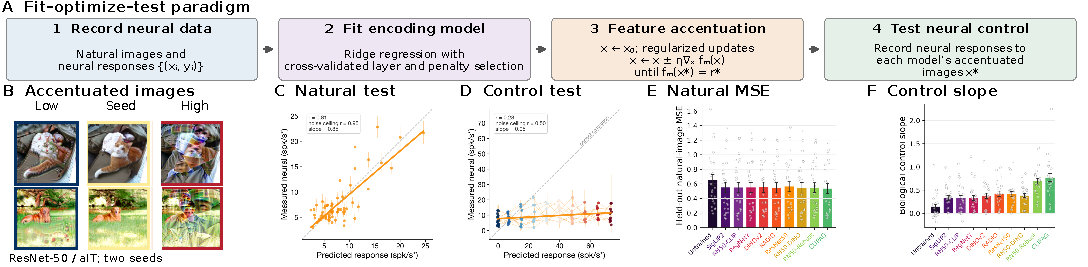
\includegraphics[width=\linewidth]{figures/cosyne2027_figure1_workflow.pdf}
\captionof{figure}{\textbf{From encoding to control.} \textbf{A}~Experimental paradigm of closed-loop model-based control comparison. \textbf{B--D}~One ResNet-50/aIT site from~[1]: two accentuation sweeps; natural test responses ($r=0.81$, slope $0.85$); control responses ($r=0.28$, slope $0.05$). \textbf{E,F}~Natural-image MSE and control slope across ten models: sites (dots), mean and $\pm1$~SE (bars); 25 sites.}
\label{fig:experiment}
\end{minipage}\par

\head{From experiment to a solvable model.}
We preserve the backbone--readout structure but replace $\phi(x)$ by fixed linear features $Fx$. Natural inputs $x\sim\mathcal N(0,\Sigma)$ drive a noisy linear neuron, $y=x^\top\bt+\sigma\epsilon$, with independent unit-variance noise $\epsilon$ and signal variance $S={\bt}^\top\Sigma\bt$. Ridge regression on $n$ examples fits $f(x)=\hat w^\top Fx=x^\top\bh$, with pixel gradient $\bh=F^\top\hat w$ (Fig.~\ref{fig:evidence}A). We retain ridge fitting but idealize regularized synthesis as the straight path $x=x_0+\alpha\bh$. With $x_0=0$ and a centered sweep $\mathbb E[\alpha]=0$, mean neural and predicted response changes are $\alpha N$ and $\alpha D$:
\begin{equation}
\mathrm{slope}_{\rm control}=\frac ND=
\frac{\bh^\top\bt}{\|\bh\|^2}\,
\begin{subarray}{l}
\text{actual neural gain}\\[4pt]
\text{model-predicted gain}
\end{subarray},
\qquad R^2_{\rm control}=1-\left(\frac DN-1\right)^2.
\label{eq:geometry}
\end{equation}
Alignment $N$ is the actual neural gain; squared norm $D$ is the model's claimed gain. For $N>0$, $D<N$ means underprediction (slope $>1$), $D=N$ means perfect calibration, and $D>N$ means overprediction (slope $<1$), which could lead to negative $R^2$ (when $D>2N$). Natural-image prediction instead measures $E_{\rm gen}=(\bh-\bt)^\top\Sigma(\bh-\bt)$, downweighting low-variance directions. Errors along these directions can therefore inflate the model's claimed gain $D$ with little predictive cost or corresponding neural gain $N$.

\head{Why cross-validation does not remove the problem.}
The failure already occurs for $F=I$, with no backbone geometry. Random matrix theory~[3] gives leading approximations as dimension and sample size grow proportionally. The mean weight is the teacher shrunk along each covariance eigenvector:
\begin{equation}
\mb:=\Sigma(\Sigma+\kappa I)^{-1}\bt
=\sum\nolimits_k\frac{s_k}{s_k+\kappa}\,b_k u_k,
\qquad \Sigma u_k=s_k u_k,\quad b_k=u_k^\top\bt.
\label{eq:mean-shrinkage}
\end{equation}
Here $\kappa$ is the effective ridge penalty accounting for finite sampling; each shrinkage factor $s_k/(s_k+\kappa)\in[0,1]$.\par
Finite-data fluctuations inflate squared norm $D$ by $V$, without changing leading alignment $N$:
\begin{equation}
\mathrm{slope}_{\rm control}\simeq
\frac{\mb^\top\bt}{\|\mb\|^2+V},
\qquad
V=\frac{E_{\rm gen}+\sigma^2}{n}
\sum\nolimits_k\frac{s_k}{(s_k+\kappa)^2},
\label{eq:inflation}
\end{equation}\par
For the mean alone, $\|\mb\|^2\le\mb^\top\bt$: the student underpredicts. Inflation increases the model-predicted gain $D$ without increasing the neural gain $N$. It first compensates for shrinkage, giving $D=N$, then causes overprediction once $D>N$. For independent ridge fits, $V$ drops out of the peer weight cross-product, yielding shrinkage-driven underprediction, consistent with neural data (Fig.~\ref{fig:evidence}E).\par
Prediction-optimal and control-calibrated penalties satisfy different spectral conditions for anisotropic inputs and a structured teacher. Natural-image simulations exhibit distinct optima (Fig.~\ref{fig:evidence}B): selecting a penalty for prediction need not calibrate control.\par

\head{Why equally predictive feature maps control differently.}
For general $F$, prediction depends on $F\Sigma F^\top$ and $h=F\Sigma\bt$, with signal variance, noise and sample size fixed; control also depends on $FF^\top$ and $F\bt$. We construct transformations preserving the joint feature--response distribution, hence the predicted generalization curve and its optimal penalty stay invariant, while control changes (Fig.~\ref{fig:evidence}C). Increasing input anisotropy can make this dissociation arbitrarily severe.

The feature-gradient geometry enters the norm inflation, 
\begin{equation}
V_F=\frac{E_{\rm gen}+\sigma^2}{n}\,T_F(\kappa),
\qquad
T_F(\kappa)=\sum\nolimits_{k:s_k>0}
\left(\frac{s_k}{s_k+\kappa}\right)^2
\frac{\|g_k\|^2}{g_k^\top\Sigma g_k},
\label{eq:features}
\end{equation}
where $(s_k,v_k)$ now denote feature-covariance eigenpairs and $g_k=F^\top v_k$ is a feature direction's pixel gradient. The sum weights features that survive regularization and compares their gradient energy with natural-image variation along that gradient. Thus, control is fragile when well-estimated features send their gradients into weakly constrained pixel directions, making $T_F$ large without changing prediction error.

\head{From linear theory to biological control.}
For nonlinear features $\phi$, the feature Jacobian $J_\phi$ at seed images gives $T_\phi=\sum\nolimits_k s_k/(s_k+\kappa)^2\|J_\phi(x)^\top v_k\|^2$. Averaging squared gradients over a Gaussian input neighborhood (standard deviation $16/255$) and scaling by held-out mean squared error (MSE) divided by $n$ gives a neighborhood inflation proxy $V_\phi$. Across nine trained models and 25 sites (225 pairs), raw $\log_{10}$ predictors correlate with site-centered control slope at $r=-0.61$ for $T_\phi$, $-0.54$ for neighborhood $V_\phi$, and $0.02$ for held-out MSE (Fig.~\ref{fig:evidence}D). Site means are computed over all ten models before excluding the untrained baseline. These descriptive associations support assessing gradient geometry alongside prediction accuracy.

\par\noindent\begin{minipage}{\linewidth}\centering
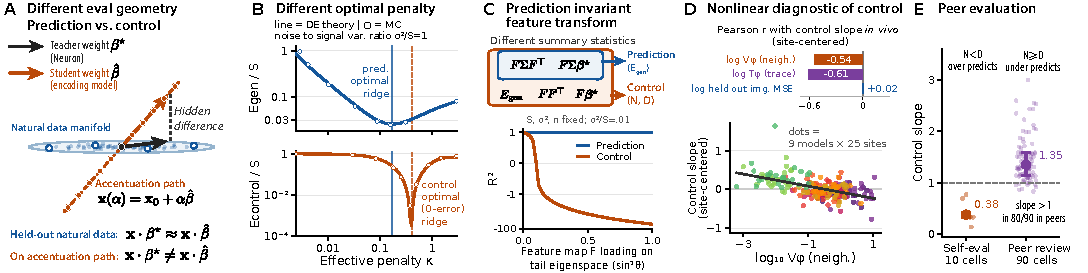
\includegraphics[width=\linewidth]{figures/cosyne2027_v19_figure2_manual.pdf}
\captionof{figure}{\textbf{Prediction--control dissociation.} \textbf{A}~Weight errors along low-variance data modes exposed by accentuation. \textbf{B}~Distinct optimal ridge penalties. \textbf{C}~Prediction and control have different summary statistics; Feature transform can change control without touching prediction. \textbf{D}~Log-predictor correlations with site-centered slope (nine models, 25 sites). \textbf{E}~Site-averaged self/peer slopes; bars: median and interquartile range.}
\label{fig:evidence}
\end{minipage}\par

\head{Toward more reliable neural control.}
The factorization $V_F=(E_{\rm gen}+\sigma^2)T_F/n$ turns the failure mechanism into a design guide: improve predictive fits, collect more training images, and average trials or denoise responses. At fixed effective penalty, $T_F$ adds a distinct criterion: among comparably predictive backbones, favor or regularize gradients that place less energy in low-variance image directions. The nonlinear diagnostic makes this criterion testable before synthesis. Reducing inflation addresses overprediction; calibration still requires balancing it against shrinkage. The design target is calibrated gain: optimized images should change neural responses by as much as the model predicts.

\vspace{2pt}
{\fontsize{10}{11}\selectfont
\textbf{References.}
[1] Prince, Wang, et al. (2026). Parametric neural control differentiates top neural network models of primate visual cortex. \emph{bioRxiv}, doi:10.64898/2026.08.16.745063.
[2] Hamblin et al. (2024). Feature accentuation: Revealing `what' features respond to in natural images. arXiv:2402.10039.
[3] Dobriban \& Wager (2018). High-dimensional asymptotics of prediction: Ridge regression and classification. \emph{Annals of Statistics} 46:247--279.
\par}
\end{document}
